%!TEX root = ../dokumentation.tex

%TODO: Einleitung überarbeiten
\chapter{Implementation}\label{cha:Implementation}

In the project \myCite{project} an example to simulate shaders in the graphics pipeline is implemented. The simulation and the shaders are written in C\#. The shaders are translated to GLSL which is then run on the GPU within a OpenGL program.

C\# is supported by multiple debugging frameworks including the  VisualStudio Debugger which has a broad spectrum of tools. \myCite{Microsoft_debugger.2019} GLSL is the main shader language for OpenGL which is one of the most used graphics frameworks. \myCite{Nvidia_opengl.2019}
Another reason those languages and frameworks are chosen is that I personally am very accustomed to them.

By writing the code in C\# all debugging features coming with VisualStudio can be used for the simulated shaders.

The project is a proof of concept where a basic functionality of the vertex shader and the fragment shader can be used and simulated. Only the necessary steps for using these two kinds of shaders are implemented on the simulated graphics pipeline. In addition to these necessary steps the option to activate the depth test is implemented to allow basic 3d applications.

\paragraph{Structure of a shader in C\#}

A shader is written as a class inheriting necessary features from a base class "Shader".

The base class shader has following features:
\begin{itemize}
\item An abstract "Main" function which acts as the entry point for each shader and has to be implemented in the different shaders.
\item an implementation of the different mathematical functions necessary for the basic examples.
\item A method which allows to set the value of a property within the shader class by passing its name as a string and the value as a generic type. The properties are found and the value is set by acessing it via reflections. This method also gets an attribute type to be able to check if the property has a specific custom attribute attached to it. This is to be able to differentiate between a property emulating a "in" or a "uniform" variable.
\item A method to return the names and values of all properties having a custom attribute of the type "OutAttribute" attached to them. These properties are found by using reflections.
\end{itemize}

To implement the different behaviors of a vertex and a fragment shader, the resulting shaders are not directly inheriting the Shader class but one of two additional abstract classes implementing the base class "Shader":
\begin{itemize}
\item The "VertexShader" class having an additional property named "Position" to emulate the built-in variable "gl\_Position" GLSL has \myCite{Khronos_builtIn.2015}. This ensures the vertex shader to always return a position value for the output vertex.
\item The "fragmentShader" class having an additional property named "Color" with a "OutAttribute" attached to it so there is always a Color variable to draw the fragments.
\end{itemize}

\paragraph{Translation of the shader class}

The shader class is contained within a single file. To translate it, the path to this file is given to the translator which will extract the syntax tree from the shader class. The different nodes are translated according to their type and defined translation rules.

The syntax for different nodes is implemented manually for these node types.

For each identifier within the nodes of the syntax tree, it is checked if a "TranslationAttribute" defining a term to replace it with exists. If this is not the case the identifier will be directly transfered to the shader code.

Within the C\# code the different parts can have a "TranslationAttribute" attached to them containing a string with the term that this part should be replaced when being translated.

There are special patterns in the GLSL code that have no direct equivalent within C\#. The following solutions are within the project:
\begin{itemize}
\item Each GLSL shader has a line at the top defining its version. This line is simply added at the beginning of each translated shader and not emulated within the C\# version of the shader.
\item each variable within a shader can have an accessor defining if it is a writable attribute, a readable attribute or a uniform variable. This behavior is mimicked by having properties in the C\# shader class that can have one of the three custom attribute classes "InAttribure", "OutAttribute" or "uniformAttribute" attachet to them. This attribute is replaced by the corresponding "in", "out" or "uniform" tag when being translated to GLSL.
\end{itemize}

\paragraph{Implementation of the variable types}

To run the shader within the pipeline the code within it has to be functional. For this reason the different variable types with theit functionality have to be implemented in C\#. For this project the implementation is limited on the variable types "vec2", "vec3", "vec4" and "mat4". For each of these a equivalent is implemented. By implementing them as structs instead of classes the value based behavior they have in the GLSL code is reconstructed. These structs are implemented based on float values like their GLSL counterparts. The different forms of accessing their values are implemented in the form of properties and the necessary operators for the mathematical calculations with them are added.

\paragraph{Simulating the pipeline}

The stages are implemented with the functionalities described in \autoref{section:contribution_simulating}.

The application is ment to be a simple example for debugging basic shaders and thereby does not support all features. Following limitations are in the project:
\begin{itemize}
\item The primitive type is hardcoded for the use of triangle primitives only. Triangle is the most used primitive type and is sufficient to render working examples.
\item The application always runs for a default viewport spanning the whole output size of the application and does not implement viewport transformation.
\item The depth buffer and the use of depth filtering are implemented for handling basic 3D applications. A stencil buffer is not implemented and the use of stencils is not supported in the project.
\item The fragment shader always returns a color value so the application always has a graphical output.
\end{itemize}

Within the pipeline the attributes and uniforms for the shaders are set and the output values gained by using the methods implemented within the base "Shader" class. The exception is the "Position" property of the vertex shader which is accessed directly and used for the interpolation within the pipeline.

The final result is written into a "Bitmap" variable.

\paragraph{Surrounding structure}

The application is running within the OpenGL game loop.

The geometry to be rendered is prepared and manipulated in the update loop.

Within the render loop the data for the render process is genereted and then either drawn by having the translated shaders run on the GPU or given to the simulated pipeline which is then executed and returns a Bitmap variable that is then rendered as a texture on a screen filling quad.

\paragraph{Used example geometry and shaders}

For a basic example a scene consisting out of a tetrahedron which is rendered in 3 instances is chosen. These instances get different color and different transformations as shown in  \autoref{fig:exampleScene}.

The example for a vertex shader is applying the instance transformation to the vertex position and to its normal, applying a camera transformation to the resulting position and passing through the instance color.

The example for the fragment shader receives the position, the normal and the instance color and applies a light calculation based on a given directional light and the camera position.

\begin{figure}[h!]
  \centering 
  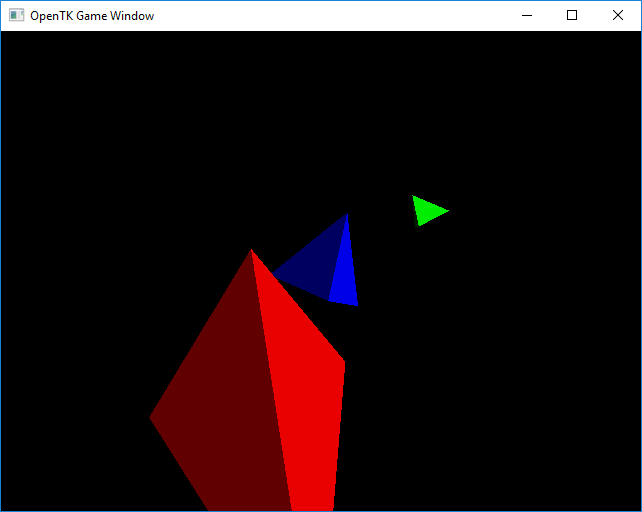
\includegraphics[scale=0.6]{scene.png}
  \caption[Screenshot of example scene of the project]{Project scene}
  \label{fig:exampleScene}
\end{figure}